% !TEX root = NSF_SuperCDMS_SNOLAB_OPS.tex

\section{Schedule}
\label{sec:schedule}

Figure~\ref{fig:ops-schedule} gives a broad view of the activities of the \SuperCDMS collaboration  centered on the \scs experiment, including the DOE/NSF G2 Project, the pre-operations and commissioning period covered by this proposal, the actual operation of \scs (also detailed in the Experimental Operations Plan), and the R\&D program that will naturally lead to upgrades for \scs that allow it to probe the low-mass dark matter region down to the neutrino floor.

% The detailed schedule for this proposal is shown in Figure~\ref{fig:ops-schedule}. 

% \begin{figure}[htb]
% \begin{center}
% 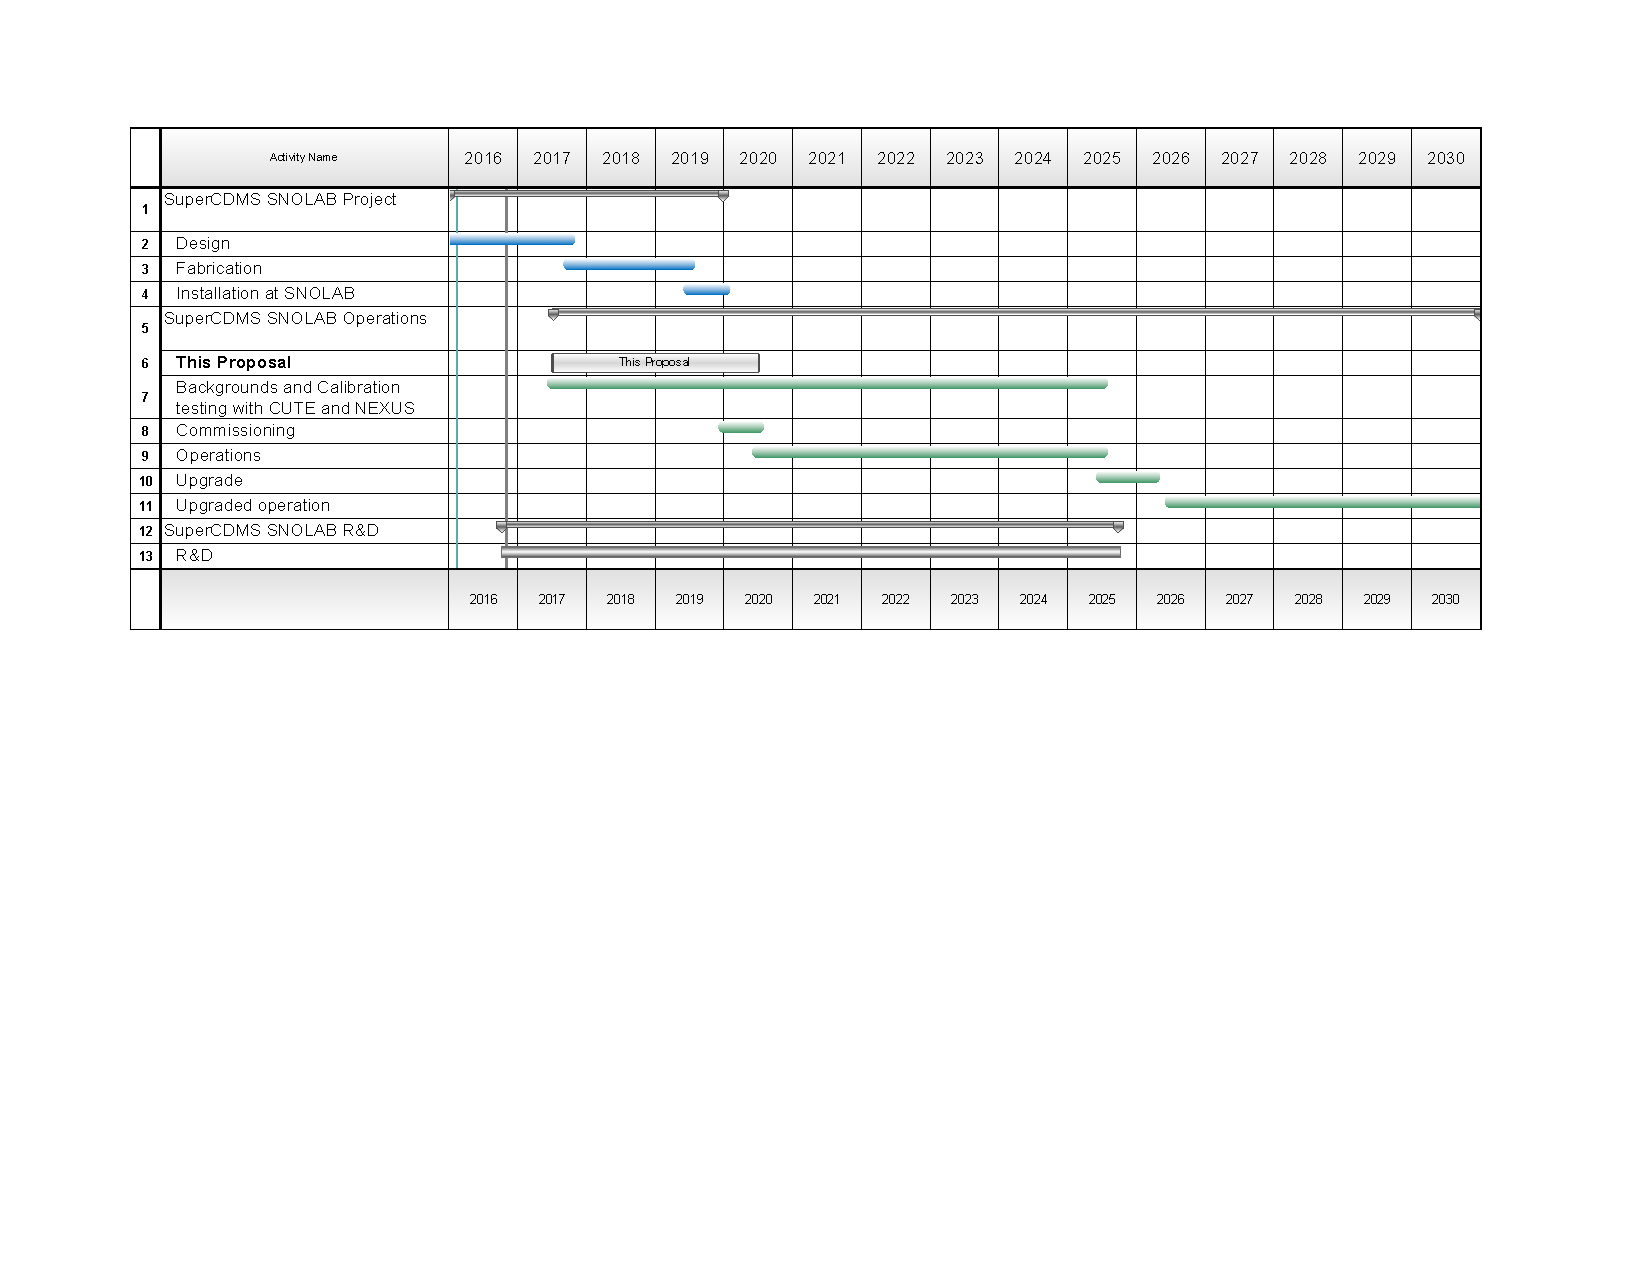
\includegraphics[width=\textwidth]{Figures/supercdms_operations_schedule_nsf_ops.pdf}
% \end{center}
% \caption{\footnotesize First draft of an interleaved schedule for the \scs Project, Operations and R$\&$D and Upgrades.}
% \label{fig:proj-schedule}
% \end{figure}

\begin{figure}[htb]
\begin{center}
  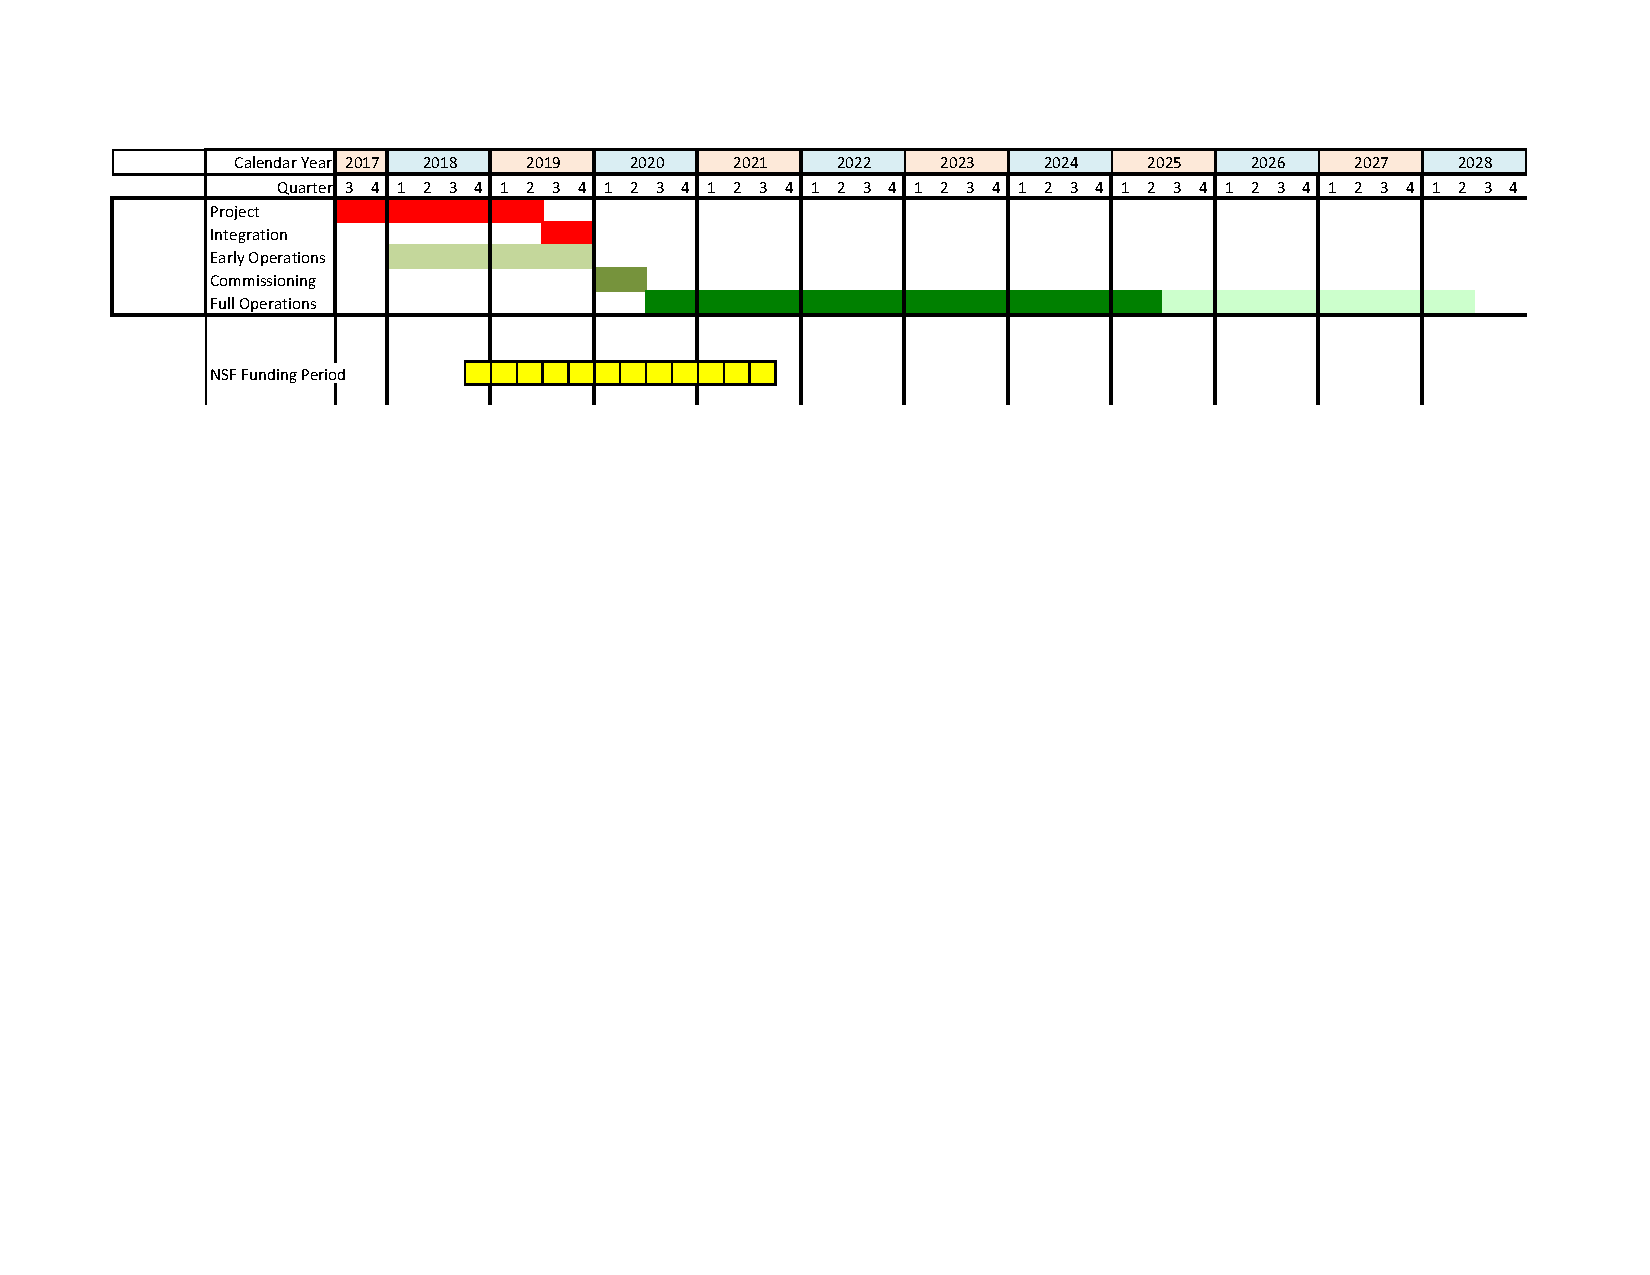
\includegraphics[width=\textwidth]{Figures/OpsSched-rac.pdf}
\end{center}
\caption{Schedule for the \scs Experiment.}
\label{fig:ops-schedule}
\end{figure}

\noindent\textbf{Year 1: 7/2018--6/2019}\\
During the first year the focus will be on calibration of the small HV test detectors from Stanford University with the Northwestern ADR at \tunl. These detectors will then be taken to \nexus, to perform cross-calibration measurements in preparation for the large detector calibrations. The first pre-production detectors arrive at \cute in January 2018, and the performance  and background measurement campaign begins soon after. 

\noindent\textbf{Year 2: 7/2019--6/2020}\\
The second year is dominated by runs of pre-production detectors at \nexus for calibration and at \cute for performance testing and background measurements. The first production \scs HV tower arrives at \cute in 12/2018, with testing commencing in 1/2019. Performance and run optimization of all six detectors of the HV tower will continue until 6/2020.

 \noindent\textbf{Year 3: 7/2020--6/2021}\\
There is no activity planned for \nexus on this grant in the third year. At \cute, the \scs HV tower science run will be taking data until 11/2019, when the tower will be taken out of \cute to prepare it for installation in the \scs experiment. Commissioning activities for \scs will be the main focus of this grant in the last six months of the award, along with the collaboration-wide effort in analysis and publication of all the data products from this work.
